\documentclass[fleqn]{article}
\usepackage[nodisplayskipstretch]{setspace}
\usepackage{amsmath, nccmath, bm}
\usepackage{amssymb}
\usepackage{enumitem}
\usepackage{graphicx}
\usepackage{float}
\usepackage{caption}

\newcommand{\zerodisplayskip}{
	\setlength{\abovedisplayskip}{0pt}%
	\setlength{\belowdisplayskip}{0pt}%
	\setlength{\abovedisplayshortskip}{0pt}%
	\setlength{\belowdisplayshortskip}{0pt}%
	\setlength{\mathindent}{0pt}}
	
\newcommand{\norm}[1]{\left \lVert #1 \right \rVert}

\makeatletter
	\newenvironment{equationCenter}{\@fleqnfalse\begin{equation*}}{\end{equation*}}
\makeatother

\title{Final Exam}
\author{Owen Sowatzke}
\date{December 12, 2024}

\begin{document}

	\offinterlineskip
	\setlength{\lineskip}{12pt}
	\setcounter{MaxMatrixCols}{20}
	\zerodisplayskip
	\maketitle
	
	\begin{enumerate}
		\item In Figure 1 is shown a $2 \times 2$ polarization-time coding MIMO scheme, which employs dual-polarization transmit and receive antennas. Due to multipath effect, the initial orthogonality of polarization states is no longer preserved on a receiver side and we can use the channel coefficients as shown in Fig. 1 to describe this depolarization effect. Show that Alamouti $2 \times 2$ scheme can be used to deal with depolarization effect. Determine the array, diversity and multiplexing gains of this scheme. How would you determine the channel capacity of this scheme? Consider now a MIMO scheme employing two dual-polarization Tx antennas and two dual-polarization Rx antennas. How would approach this system to deal simultaneously with depolarization and multipath effects? How would you determine the channel capacity of this scheme?

		\begin{figure}[H]
			\centerline{\fbox{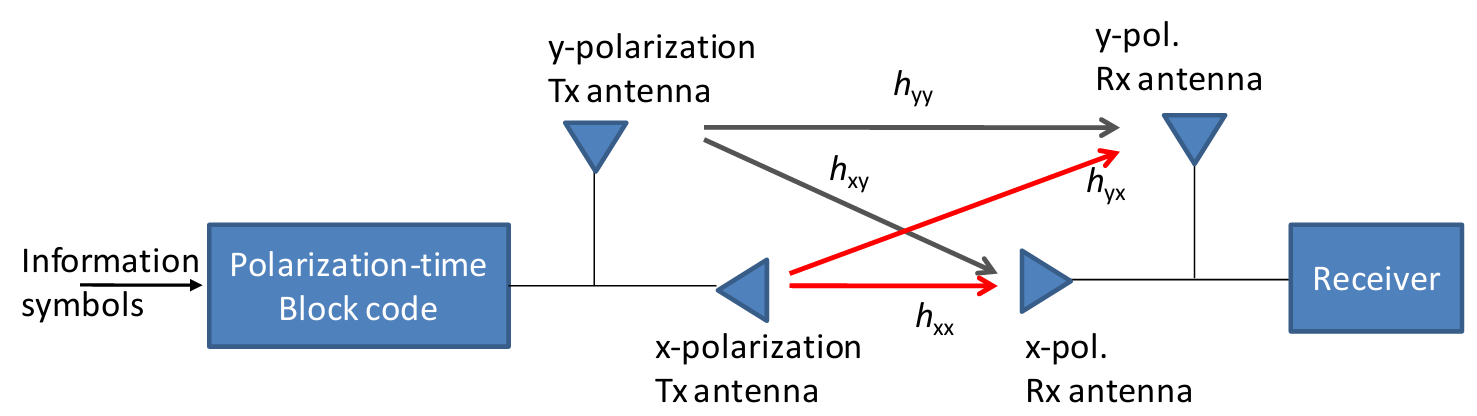
\includegraphics[width=0.8\textwidth]{2x2_polarization_time_coding_mimo.png}}}
			\caption{}
			\label{fig::2x2_polarization_time_coding_mimo}
		\end{figure}
		
%		In a MIMO system, the Alamouti $2\times 2$ scheme is implemented using the following code matrix:
%		
%		\begin{equation*}
%			\mathbf{X} = \begin{bmatrix}
%				x_1 & -x_2^*\\
%				x_2 & x_1^*
%			\end{bmatrix}
%		\end{equation*}
%		
%		In the first channel use, the antenna $T_{x_1}$ transmits $x_1$, and the antenna $T_{x_2}$ transmits $x_2$. In the second channel use, the antenna $T_{x_1}$ transmits $-x_2^*$ and the antenna $T_{x_2}$ transmits $x_1^*$.
%		
%		For a dual polarization system, we can leverage the Alamouti in a similar manner to determine to deal with the depolarization effect. In the first channel use, we send $s_x$ on the the x-polarization antenna and $s_y$ on the y-polarization antenna. In the second channel use, we send $-s_y^*$ on the x-polarization antenna and $s_x^*$ on the y-polarization antenna.
%		
%		The received signal vectors for the first and second channel use are denoted as $\mathbf{r_{i,1}}$ and $\mathbf{r_{i,2}}$ and are denoted as follows:
%		
%		\begin{equation*}
%			\mathbf{r_{i,1}} = \mathbf{Hs_{i,1}}e^{j(\phi_T - \phi_{LO}) + j\phi_{CD}(k)}
%		\end{equation*}
%		
%		\begin{equation*}
%			\mathbf{r_{i,2}} = \mathbf{Hs_{i,2}}e^{j(\phi_T - \phi_{LO}) + j\phi_{CD}(k)}
%		\end{equation*}\\
%		
%		 The transmitted symbols are now denoted as $s_x$ and $s_y$, and we use $\mathbf{S}$ to denote the code matrix.
%		
%		\begin{equation*}
%			\mathbf{S} = \begin{bmatrix}
%				s_x & -s_y^*\\
%				s_y & s_x^*
%			\end{bmatrix}
%		\end{equation*}
%		
%		FUCK
%		
%		\pagebreak
		
		\begin{equation*}
			\begin{bmatrix}
				r_{x,1} & r_{x,2} \\
				r_{y,1} & r_{y,2}
			\end{bmatrix} = \begin{bmatrix}
				h_{xx} & h_{xy} \\
				h_{yx} & h_{yy}
			\end{bmatrix}\begin{bmatrix}
				s_x & -s_y^* \\
				s_y & s_x^*
			\end{bmatrix} + \begin{bmatrix}
				n_{x,1} & n_{x,2} \\
				n_{y,1} & n_{y,2}
			\end{bmatrix}
		\end{equation*}
			
		\begin{equation*}
				 = \begin{bmatrix}
				h_{xx}s_x + h_{xy}s_y & -h_{xx}s_y^* + h_{xy}s_x^* \\
				h_{yx}s_x + h_{yy}s_y & -h_{yx}s_y^* + h_{yy}s_x^*
			\end{bmatrix} + \begin{bmatrix}
				n_{x,1} & n_{x,2} \\
				n_{y,1} & n_{y,2}
			\end{bmatrix}
		\end{equation*}
		
		We can estimate the transmitted symbols as follows:
		
		\begin{equation*}
			\tilde{s}_x = h_{xx}^*r_{x,1} + h_{xy}r_{x,2}^* + h_{yx}^*r_{y,1} + h_{yy}r_{y,2}^*
		\end{equation*}
		
		\begin{equation*}
			\tilde{s}_y = h_{xy}^*r_{x,1} - h_{xx}r_{x,2}^* + h_{yy}^*r_{y,1} - h_{yx}r_{y,2}^*
		\end{equation*}
		
		Substituting, we obtain:
		
		\begin{equation*}
			\tilde{s}_x = h_{xx}^*(h_{xx}s_x + h_{xy}s_y) + h_{xy}(-h_{xx}^*s_y + h_{xy}^*s_x) + h_{yx}^*(h_{yx}s_x + h_{yy}s_y)
		\end{equation*}
		
		\begin{equation*}
			 + h_{yy}(-h_{yx}^*s_y + h_{yy}^*s_x) + \text{noise}
		\end{equation*}
		
		\begin{equation*}
			= |h_{xx}|^2s_x + h_{xx}^*h_{xy}s_y - h_{xx}^*h_{xy}s_y + |h_{xy}|^2s_x + |h_{yx}|^*s_x + h_{yx}^*h_{yy}s_y
		\end{equation*}
		
		\begin{equation*}
			- h_{yx}^*h_{yy}s_y + |h_{yy}|^2s_x + \text{noise}
		\end{equation*}
		
		\begin{equation*}
			= (|h_{xx}|^2 + |h_{xy}|^2 + |h_{yx}|^2 + |h_{xy}|^2)s_x + \text{noise}
		\end{equation*}
		
		\begin{equation*}
			\tilde{s}_y = h_{xy}^*r_{x,1} - h_{xx}r_{x,2}^* + h_{yy}^*r_{y,1} - h_{yx}r_{y,2}^*
		\end{equation*}
		
		\begin{equation*}
			= h_{xy}^*(h_{xx}s_x + h_{xy}s_y) - h_{xx}(-h_{xx}^*s_y + h_{xy}^*s_x) + h_{yy}^*(h_{yx}s_x + h_{yy}s_y)
		\end{equation*}
		
		\begin{equation*}
			- h_{yx}(-h_{yx}^*s_y + h_{yy}^*s_x) + \text{noise}
		\end{equation*}
		
		\begin{equation*}
			= h_{xx}h_{xy}^*s_x + |h_{xy}|^2s_y + |h_{xx}|^2s_y - h_{xx}h_{xy}^*s_x + h_{yx}h_{yy}^*s_x + |h_{yy}|^2s_y
		\end{equation*}
		
		\begin{equation*}
			+ |h_{yx}|^2s_y - h_{yx}h_{yy}^*s_x + \text{noise}
		\end{equation*}
		
		\begin{equation*}
			= (|h_{xx}|^2 + |h_{xy}|^2 + |h_{yx}|^2 + |h_{yy}|^2)s_y + \text{noise}
		\end{equation*}
		
		Looking at $\tilde{s}_x$ and $\tilde{s}_y$, we can see that the Alamouti $2\times 2$ scheme effectively deals with the depolarization effect.
		
		\item An $(n,k)$ linear block code is described by the following parity-check matrix:
		
		\begin{equationCenter}
			\mathbf{H} = \begin{bmatrix}
				0 & 0 & 0 & 0 & 0 & 0 & 0 & 1 & 1 & 1 & 1 & 1 & 1 & 1 & 1 \\
				0 & 0 & 0 & 1 & 1 & 1 & 1 & 0 & 0 & 0 & 0 & 1 & 1 & 1 & 1 \\
				0 & 1 & 1 & 0 & 0 & 1 & 1 & 0 & 0 & 1 & 1 & 0 & 0 & 1 & 1 \\
				1 & 0 & 1 & 0 & 1 & 0 & 1 & 0 & 1 & 0 & 1 & 0 & 1 & 0 & 1
			\end{bmatrix}
		\end{equationCenter}
		
		\begin{enumerate}
			\item Determine the code parameters of this code: codeword length, number of information bits, code rate, overhead, minimum distance, error correction capability, and error detection capability.
			
			$\mathbf{H}$ is a $(n-k) \times n$ matrix.

			$\Rightarrow n = 15,\ k = 11$
						
			Codeword length: $n = 15\ \text{bits}$
			
			Number of information bits: $k = 11\ \text{bits}$
			
			Code rate: $R = k/n = 11/15$
			
			Overhead: $n - k = 4\ \text{bits}$
			
			The minimum distance of a linear block code is defined by the minimum number of columns of the $\mathbf{H}$-matrix whose sum is equal to the zero vector:
			
			Minimum distance: $d_\text{min} = 7$
			
			Error correction capability and error detection capability are related to the minimum distance by
			
			\begin{equation*}
				d_{\text{min}} = \geq e_d + e_c + 1
			\end{equation*}
			
			where $e_d$ is the number of detected errors and $e_c$ is the number of corrected errors.
			
			To determine error correction capability, we must set $e_d = e_c$ because we must detect the errors in all the bits we correct.
			
			\begin{equation*}
				\Rightarrow d_{\text{min}} \geq 2e_c + 1 \Rightarrow 2e_c \leq d_{\text{min}} - 1 \Rightarrow e_c \leq 3
			\end{equation*}
			
			$\therefore$ we can correct up to 3 bits in error.
			
			To determine error detection capability, we must set $e_c = 0$ because we are only responsible for detecting errors.
			
			\begin{equation*}
				\Rightarrow d_{\text{min}} \geq e_d + 1 \Rightarrow e_d \leq d_{\text{min}} - 1 \Rightarrow e_d \leq 6
			\end{equation*}
			
			$\therefore$ we can detect up to 6 bits in error.
			
			%\begin{equation*}

			\item Represent the $\mathbf{H}$-matrix in systematic form and determine the generator matrix $\mathbf{G}$ of the corresponding systematic code. Provide the corresponding shift register based encoding circuit of this systematic code.
			
			The systematic form of $\mathbf{H}$ is given as follows:
			
			\begin{equation*}
				\mathbf{H} = \left[\begin{array}{c|c}
					\mathbf{P^T} & \mathbf{I}
				\end{array}\right]
			\end{equation*}
			
			We should be able to use row operations and column permutations to put $\mathbf{H}$ in the requested form. The columns of $\mathbf{H}$ that form an identity matrix are already present. Using column permutations, we can find the systematic form, which is given below:
			
			\begin{equation*}
				\mathbf{H} = \begin{bmatrix}
					0 & 0 & 0 & 0 & 1 & 1 & 1 & 1 & 1 & 1 & 1 & 1 & 0 & 0 & 0 \\
					0 & 1 & 1 & 1 & 0 & 0 & 0 & 1 & 1 & 1 & 1 & 0 & 1 & 0 & 0 \\
					1 & 0 & 1 & 1 & 0 & 1 & 1 & 0 & 0 & 1 & 1 & 0 & 0 & 1 & 0 \\
					1 & 1 & 0 & 1 & 1 & 0 & 1 & 0 & 1 & 0 & 1 & 0 & 0 & 0 & 1
				\end{bmatrix}
			\end{equation*}
		
			The systematic generator matrix $\mathbf{G}$ is now given as follows:
			
			\begin{equation*}
				\mathbf{G} = \left[\begin{array}{c|c}
					\mathbf{I} & \mathbf{P}
				\end{array}\right]
			\end{equation*}
			
			\begin{equation*}
				\mathbf{G} = \begin{bmatrix}
					1 & 0 & 0 & 0 & 0 & 0 & 0 & 0 & 0 & 0 & 0 & 0 & 0 & 1 & 1\\
					0 & 1 & 0 & 0 & 0 & 0 & 0 & 0 & 0 & 0 & 0 & 0 & 1 & 0 & 1\\
					0 & 0 & 1 & 0 & 0 & 0 & 0 & 0 & 0 & 0 & 0 & 0 & 1 & 1 & 0\\
					0 & 0 & 0 & 1 & 0 & 0 & 0 & 0 & 0 & 0 & 0 & 0 & 1 & 1 & 1\\
					0 & 0 & 0 & 0 & 1 & 0 & 0 & 0 & 0 & 0 & 0 & 1 & 0 & 0 & 1\\
					0 & 0 & 0 & 0 & 0 & 1 & 0 & 0 & 0 & 0 & 0 & 1 & 0 & 1 & 0\\
					0 & 0 & 0 & 0 & 0 & 0 & 1 & 0 & 0 & 0 & 0 & 1 & 0 & 1 & 1\\
					0 & 0 & 0 & 0 & 0 & 0 & 0 & 1 & 0 & 0 & 0 & 1 & 1 & 0 & 0\\
					0 & 0 & 0 & 0 & 0 & 0 & 0 & 0 & 1 & 0 & 0 & 1 & 1 & 0 & 1\\
					0 & 0 & 0 & 0 & 0 & 0 & 0 & 0 & 0 & 1 & 0 & 1 & 1 & 1 & 0\\
					0 & 0 & 0 & 0 & 0 & 0 & 0 & 0 & 0 & 0 & 1 & 1 & 1 & 1 & 1
				\end{bmatrix}
			\end{equation*}
			
			The codeword is given as follows:
			
			\begin{equation*}
				\mathbf{x} = \begin{bmatrix}{\begin{array}{c|c}
					\mathbf{m} & \mathbf{b}			
				\end{array}}\end{bmatrix} = \mathbf{m}\begin{bmatrix}
					\begin{array}{c|c}
						\mathbf{I} & \mathbf{P}
					\end{array}
				\end{bmatrix} = \mathbf{mG} 
				\Rightarrow \mathbf{b} = \mathbf{mP}
			\end{equation*}
			
			The parity bits are given as follows:
			
			\begin{equation*}
				b_0 = p_{4,0}m_{4} + p_{5,0}m_{5} + p_{6,0}m_{6} + p_{7,0}m_{7} + p_{8,0}m_{8} + p_{9,0}m_{9} + p_{10,0}m_{10}
			\end{equation*}
			
			\begin{equation*}
				b_1 = p_{1,1}m_{1} + p_{2,1}m_{2} + p_{3,1}m_{3} + p_{7,0}m_{7} + p_{8,1}m_{8} + p_{9,1}m_{9} + p_{10,1}m_{10}
			\end{equation*}
			
			\begin{equation*}
				b_2 = p_{0,2}m_{0} + p_{2,2}m_{2} + p_{3,2}m_{3} + p_{5,3}m_{5} + p_{6,3}m_{6} + p_{9,3}m_{9} + p_{10,3}m_{10}
			\end{equation*}
			
			\begin{equation*}
				b_3 = p_{0,3}m_{0} + p_{1,3}m_{1} + p_{3,3}m_{3} + p_{4,3}m_{4} + p_{6,3}m_{6} + p_{8,3}m_{8} + p_{10,3}m_{10}
			\end{equation*}
			
			\item The extended code is created by inserting the additional parity-check bits. The most common way of extending the code is by adding an overall parity-check bit. The extended code is then an $(n+1,k)$ code. Determine the bipartite (Tanner) graph of $\mathbf{H}$-matrix of extended code obtained from the original $\mathbf{H}$-matrix above.
			
			We can XOR the bits of the parity matrix to add an even overall parity check-bit.
			
			\begin{equation*}
				\mathbf{P} = \begin{bmatrix}
					0 & 0 & 1 & 1 & 0 \\
					0 & 1 & 0 & 1 & 0 \\
					0 & 1 & 1 & 0 & 0 \\
					0 & 1 & 1 & 1 & 1 \\
					1 & 0 & 0 & 1 & 0 \\
					1 & 0 & 1 & 0 & 0 \\
					1 & 0 & 1 & 1 & 1 \\
					1 & 1 & 0 & 0 & 0 \\
					1 & 1 & 0 & 1 & 1 \\
					1 & 1 & 1 & 0 & 1 \\
					1 & 1 & 1 & 1 & 0
				\end{bmatrix}
			\end{equation*}
			
			The parity-check matrix is now given as follows:
			
			\begin{equation*}
				\mathbf{H} = \begin{bmatrix}
					0 & 0 & 0 & 0 & 1 & 1 & 1 & 1 & 1 & 1 & 1 & 1 & 0 & 0 & 0 \\
					0 & 1 & 1 & 1 & 0 & 0 & 0 & 1 & 1 & 1 & 1 & 0 & 1 & 0 & 0 \\
					1 & 0 & 1 & 1 & 0 & 1 & 1 & 0 & 0 & 1 & 1 & 0 & 0 & 1 & 0 \\
					1 & 1 & 0 & 1 & 1 & 0 & 1 & 0 & 1 & 0 & 1 & 0 & 0 & 0 & 1
				\end{bmatrix}
			\end{equation*}

			\item Determine the code parameters of the extended code in (c): codeword length, number of information bits, code rate, overhead, minimum distance, error correction capability, and error detection capability.
		\end{enumerate}
		
		\item This problem is related to the \textbf{adaptive modulation and coding applied to 9-ary 2-D constellation} described below, transmitted over wireless channel in the presence of Nakagami fading and AWGN. The eight constellation points in this 2-D constellation are placed on a circle of radius 1. The last (ninth) point is placed in the origin. Assume that the point in the origin appears with probability 0.5, all others with probability 0.5/8. For channel coding use the extended code from Problem 2(c).
		
		\begin{enumerate}
			\item Determine the average symbol error probability for this modulation format in the presence of fading and AWGN.
			
			\item Estimate the coding gain for the extended code from Problem 2(c) and use it in incoming (c)-(e) problems.
			
			\item Determine the optimum power adaptation strategy as well as the corresponding the spectral efficiency of this scheme, in the presence of fading and AWGN.
			
			\item Describe the channel inversion technique for this signal constellation and determine the corresponding spectral efficiency, in the presence of fading and AWGN.
			
			\item Describe the truncated channel inversion technique for this signal constellation and determine the corresponding spectral efficiency, in the presence of fading and AWGN.
		\end{enumerate}
		
		\item In this problem we are concerned with designing an OFDM system that can provide data rate $\geq 50$ Mb/s for available bandwidth of 20 MHz, and which can tolerate the delay spread of up to 100 ns. Provide the design of such a system and describe the corresponding OFDM transceiver.
		
		The guard time should be 2-4 times RMS of delay spread.
		
		Let guard time be $4\times$ RMS of delay spread.
		
		\begin{equation*}
			\Rightarrow \text{Guard Time} = \mathbf{400\ ns}
		\end{equation*}
		
		Symbol duration should be at least $5\times$ the guard time. 
		
		Let symbol duration by $5\times$ guard time
		
		\begin{equation*}
			\Rightarrow \text{Symbol Duration} = \mathbf{2\ \mu{s}}
		\end{equation*}
		
		Subcarrier spacing:
		
		\begin{equation*}
			{\Delta}f_{sc} = 1/(T_s - T_G) = \mathbf{625\ \text{\textbf{kHz}}}
		\end{equation*}
		
		Number of carriers = (the required bit rate) / (OFDM symbol rate)
		
		= (the required bit rate) * (OFDM symbol duration)
		 
		\begin{equation*}
			= 50\ \text{Mbps} \times 2\ {\mu}s = \mathbf{100\ \text{\textbf{bits per OFDM symbol}}}
		\end{equation*}
		
		Determine minimum number of bits per symbol before rate coding:
		
		\begin{equation*}
			100\ \text{bits} \times \frac{625\ \text{kHz}/\text{symbol}}{20\ \text{MHz}} = 3.125
		\end{equation*}
		
		$\Rightarrow$ At least 4 bits per symbol before rate coding. 
		
		Example rates and coding:
		
		Option 1: 16-QAM and $1/2$ rate coding: 50 subcarriers (2 bits per symbol per subcarrier)
		
		Option 2: QPSK with $3/4$ rate coding (1.5 bits per symbol per carrier): 75 subcarriers.
		
		128
		
		
		\item This problem is related to \textbf{coded-modulation applied to 9-ary 2-D constellation} described in Problem 3, in the presence of Nakagami fading and AWGN.
		
		\begin{enumerate}
			\item Describe the transmitter and receiver configuration for 9-ary LDPC-coded modulation for $2 \times 2$ MIMO system.
			
			\item Determine the symbol LLRs required for 3-ary LDPC decoding. Describe how to determine the extrinsic information at the output of 3-ary LDPC decoder for APP demapper. Describe how to determine the prior symbol LLRs for next APP-LDPC decoder iteration step.
		\end{enumerate}
	\end{enumerate}
\end{document}